\documentclass[14pt,a4paper]{article}
\pagenumbering{gobble}
\usepackage[utf8]{inputenc}
\usepackage{amsmath}
\usepackage{amsfonts}
\usepackage{amssymb}
\usepackage[T1]{fontenc}
\usepackage[utf8]{inputenc}
\usepackage{graphicx}
\usepackage{hyperref}
\usepackage[english,russian]{babel}
\usepackage[left=1cm,right=1cm,
top=1cm,bottom=2cm,bindingoffset=0cm]{geometry}

\providecommand{\tightlist}{%
	\setlength{\itemsep}{0pt}\setlength{\parskip}{0pt}}

\usepackage{color}
\usepackage{fancyvrb}
\newcommand{\VerbBar}{|}
\newcommand{\VERB}{\Verb[commandchars=\\\{\}]}
% Add ',fontsize=\small' for more characters per line
\definecolor{shadecolor}{RGB}{248,248,248}
\newenvironment{Shaded}{\begin{paragraph}}{\end{paragraph}}
\newenvironment{Highlighting}{\begin{paragraph}}{\end{paragraph}}
\newcommand{\KeywordTok}[1]{\textcolor[rgb]{0.13,0.29,0.53}{\textbf{#1}}}
\newcommand{\DataTypeTok}[1]{\textcolor[rgb]{0.13,0.29,0.53}{#1}}
\newcommand{\DecValTok}[1]{\textcolor[rgb]{0.00,0.00,0.81}{#1}}
\newcommand{\BaseNTok}[1]{\textcolor[rgb]{0.00,0.00,0.81}{#1}}
\newcommand{\FloatTok}[1]{\textcolor[rgb]{0.00,0.00,0.81}{#1}}
\newcommand{\ConstantTok}[1]{\textcolor[rgb]{0.00,0.00,0.00}{#1}}
\newcommand{\CharTok}[1]{\textcolor[rgb]{0.31,0.60,0.02}{#1}}
\newcommand{\SpecialCharTok}[1]{\textcolor[rgb]{0.00,0.00,0.00}{#1}}
\newcommand{\StringTok}[1]{\textcolor[rgb]{0.31,0.60,0.02}{#1}}
\newcommand{\VerbatimStringTok}[1]{\textcolor[rgb]{0.31,0.60,0.02}{#1}}
\newcommand{\SpecialStringTok}[1]{\textcolor[rgb]{0.31,0.60,0.02}{#1}}
\newcommand{\ImportTok}[1]{#1}
\newcommand{\CommentTok}[1]{\textcolor[rgb]{0.56,0.35,0.01}{\textit{#1}}}
\newcommand{\DocumentationTok}[1]{\textcolor[rgb]{0.56,0.35,0.01}{\textbf{\textit{#1}}}}
\newcommand{\AnnotationTok}[1]{\textcolor[rgb]{0.56,0.35,0.01}{\textbf{\textit{#1}}}}
\newcommand{\CommentVarTok}[1]{\textcolor[rgb]{0.56,0.35,0.01}{\textbf{\textit{#1}}}}
\newcommand{\OtherTok}[1]{\textcolor[rgb]{0.56,0.35,0.01}{#1}}
\newcommand{\FunctionTok}[1]{\textcolor[rgb]{0.00,0.00,0.00}{#1}}
\newcommand{\VariableTok}[1]{\textcolor[rgb]{0.00,0.00,0.00}{#1}}
\newcommand{\ControlFlowTok}[1]{\textcolor[rgb]{0.13,0.29,0.53}{\textbf{#1}}}
\newcommand{\OperatorTok}[1]{\textcolor[rgb]{0.81,0.36,0.00}{\textbf{#1}}}
\newcommand{\BuiltInTok}[1]{#1}
\newcommand{\ExtensionTok}[1]{#1}
\newcommand{\PreprocessorTok}[1]{\textcolor[rgb]{0.56,0.35,0.01}{\textit{#1}}}
\newcommand{\AttributeTok}[1]{\textcolor[rgb]{0.77,0.63,0.00}{#1}}
\newcommand{\RegionMarkerTok}[1]{#1}
\newcommand{\InformationTok}[1]{\textcolor[rgb]{0.56,0.35,0.01}{\textbf{\textit{#1}}}}
\newcommand{\WarningTok}[1]{\textcolor[rgb]{0.56,0.35,0.01}{\textbf{\textit{#1}}}}
\newcommand{\AlertTok}[1]{\textcolor[rgb]{0.94,0.16,0.16}{#1}}
\newcommand{\ErrorTok}[1]{\textcolor[rgb]{0.64,0.00,0.00}{\textbf{#1}}}
\newcommand{\NormalTok}[1]{#1}

\begin{document}

\hypertarget{ux43dux435ux441ux442ux430ux43dux434ux430ux440ux442ux43dux44bux439-ux43fux43eux43bux438ux43cux43eux440ux444ux438ux437ux43c.-ux43fux430ux442ux442ux435ux440ux43d-type-erasure.}{%
\section{Нестандартный полиморфизм. Паттерн Type
Erasure.}\label{ux43dux435ux441ux442ux430ux43dux434ux430ux440ux442ux43dux44bux439-ux43fux43eux43bux438ux43cux43eux440ux444ux438ux437ux43c.-ux43fux430ux442ux442ux435ux440ux43d-type-erasure.}}

\hypertarget{ux43eux433ux43bux430ux432ux43bux435ux43dux438ux435}{%
\section{Оглавление}\label{ux43eux433ux43bux430ux432ux43bux435ux43dux438ux435}}

\begin{itemize}
\tightlist
\item
  \protect\hyperlink{ux432ux432ux435ux434ux435ux43dux438ux435-ux438-ux43fux43eux441ux442ux430ux43dux43eux432ux43aux430-ux437ux430ux434ux430ux447ux438}{Введение
  и постановка задачи}
\item
  \protect\hyperlink{ux43dux430ux441ux43bux435ux434ux43eux432ux430ux43dux438ux435}{Наследование}
\item
  \protect\hyperlink{ux43fux430ux442ux442ux435ux440ux43dux44b}{Паттерны}
\item
  \protect\hyperlink{ux434ux432ux438ux433ux430ux435ux43cux441ux44f-ux43a-type-erasure}{Двигаемся
  к Type Erasure}

  \begin{itemize}
  \tightlist
  \item
    \protect\hyperlink{ux43fux430ux442ux442ux435ux440ux43d-external-polymorphism}{Паттерн
    External Polymorphism}
  \end{itemize}
\item
  \protect\hyperlink{type-erasure}{Type Erasure}
\item
  \protect\hyperlink{ux43fux43eux43bux43dux44bux439-ux43aux43eux434}{Полный
  код}
\item
  \protect\hyperlink{ux438ux441ux442ux43eux447ux43dux438ux43aux438}{Источники}
\end{itemize}

\hypertarget{ux432ux432ux435ux434ux435ux43dux438ux435-ux438-ux43fux43eux441ux442ux430ux43dux43eux432ux43aux430-ux437ux430ux434ux430ux447ux438}{%
\section{Введение и постановка
задачи}\label{ux432ux432ux435ux434ux435ux43dux438ux435-ux438-ux43fux43eux441ux442ux430ux43dux43eux432ux43aux430-ux437ux430ux434ux430ux447ux438}}

Посмотрим на проблему.

Решим ее обычным полиморфизмом.

Пройдем небольшими шагами к более элегантному решению.

Изменения - основная проблема создания программного обеспечения. Большая
задача в разработке ПО - сделать его таким, чтобы его можно было легко
изменять. И одной из основных проблем в изменении существующего кода -
его зависимости. Привязанность кода к внешним зависимостям очень сильно
``сковывает'' движения программиста при внесении чего-то нового в код.

Посмотрим на задачу: хотим рисовать разные фигуры.

Задача детская, скучная, но очень хорошо иллюстрирующая всё, что я
собираюсь показать.

Но не заостряйте свое внимание именно на фигурах, все-таки паттерн, про
который я собираюсь рассказать, применим еще много к чему.

\hypertarget{ux43dux430ux441ux43bux435ux434ux43eux432ux430ux43dux438ux435}{%
\section{Наследование}\label{ux43dux430ux441ux43bux435ux434ux43eux432ux430ux43dux438ux435}}

Мы хотим рисовать разные фигуры. Сперва создадим базовый абстрактный
класс \texttt{Shape} с методом его рисования на экран

\begin{Shaded}
\begin{Highlighting}
\KeywordTok{struct}\NormalTok{ Shape }\OperatorTok{\{}
    \KeywordTok{virtual} \DataTypeTok{void}\NormalTok{ draw}\OperatorTok{()} \OperatorTok{=} \DecValTok{0}\OperatorTok{;}
\OperatorTok{\};}
\end{Highlighting}
\end{Shaded}

Теперь определим парочку конкретных фигур, например квадрат и круг
унаследовав их классы \texttt{Square} и \texttt{Circle} от
\texttt{Shape}. Также в них определим виртуальный метод \texttt{draw}.

\begin{Shaded}
\begin{Highlighting}[]
\KeywordTok{struct}\NormalTok{ Circle }\OperatorTok{:} \KeywordTok{public}\NormalTok{ Shape }\OperatorTok{\{}
    \DataTypeTok{void}\NormalTok{ draw}\OperatorTok{()} \KeywordTok{override} \OperatorTok{\{}
        \BuiltInTok{std::}\NormalTok{cout}\OperatorTok{ \textless{}\textless{}} \StringTok{"I am Circle"} \OperatorTok{\textless{}\textless{}} \BuiltInTok{std::}\NormalTok{endl}\OperatorTok{;}
    \OperatorTok{\}}
\OperatorTok{\};}

\KeywordTok{struct}\NormalTok{ Square }\OperatorTok{:} \KeywordTok{public}\NormalTok{ Shape }\OperatorTok{\{}
    \DataTypeTok{void}\NormalTok{ draw}\OperatorTok{()} \KeywordTok{override} \OperatorTok{\{}
        \BuiltInTok{std::}\NormalTok{cout}\OperatorTok{ \textless{}\textless{}} \StringTok{"I am Square"} \OperatorTok{\textless{}\textless{}} \BuiltInTok{std::}\NormalTok{endl}\OperatorTok{;}
    \OperatorTok{\}}
\OperatorTok{\};}
\end{Highlighting}
\end{Shaded}

Типов фигур может быть очень много, каждый из классов фигур обязан
давать определение методу \texttt{draw}. Но такой подход может очень
быстро привести нас к проблемам.

Рассмотрим конкретный класс \texttt{Circle} - в нашей текущей реализации
он сильно связан с деталями реализации механизма рисования фигур на
экран, а это плохо.

Например, реализация рисования фигур может быть зашита где-то глубоко в
используемой библиотеке или написана в другом месте проекта.

К тому же такой подход позволяет иметь только одну реализацию рисования
фигур. Допустим, мы пишем приложение, использую OpenGL для рисования
разной информации на экран, но вдруг нам понадобилось портировать весь
рисующий функционал ещё и на Vulkan/Metal/DirectX. Что делать в таком
случае? К решению этой проблемы можно подойти с разных сторон.

Первый подход - добавить новые методы рисования:

\begin{Shaded}
\begin{Highlighting}[]
\KeywordTok{struct}\NormalTok{ Shape }\OperatorTok{\{}
    \KeywordTok{virtual} \DataTypeTok{void}\NormalTok{ drawOpenGL}\OperatorTok{()} \OperatorTok{=} \DecValTok{0}\OperatorTok{;}
    \KeywordTok{virtual} \DataTypeTok{void}\NormalTok{ drawVulkan}\OperatorTok{()} \OperatorTok{=} \DecValTok{0}\OperatorTok{;}
    \CommentTok{// и так далее}
\OperatorTok{\};}
\end{Highlighting}
\end{Shaded}

Тогда при использовании данного класса нам нужно будет делать выбор,
какой из методов использовать:

\begin{Shaded}
\begin{Highlighting}[]
\DataTypeTok{void}\NormalTok{ drawAll}\OperatorTok{(}\BuiltInTok{std::}\NormalTok{vector}\OperatorTok{\textless{}}\NormalTok{Shape}\OperatorTok{*\textgreater{}}\NormalTok{ v}\OperatorTok{)\{}
    \ControlFlowTok{for}\OperatorTok{(}\KeywordTok{auto} \OperatorTok{*}\NormalTok{shape}\OperatorTok{:}\NormalTok{ v}\OperatorTok{)\{}
        \ControlFlowTok{switch} \OperatorTok{(}\NormalTok{API}\OperatorTok{::}\NormalTok{getGraphicsApi}\OperatorTok{())} \OperatorTok{\{}
            \ControlFlowTok{case}\NormalTok{ OpenGL}\OperatorTok{:}
\NormalTok{                shape}\OperatorTok{{-}\textgreater{}}\NormalTok{drawdrawOpenGL}\OperatorTok{();}
                \ControlFlowTok{break}\OperatorTok{;}
            \ControlFlowTok{case}\NormalTok{ Vulkan}\OperatorTok{:}
\NormalTok{                shape}\OperatorTok{{-}\textgreater{}}\NormalTok{drawVulkan}\OperatorTok{();}
                \ControlFlowTok{break}\OperatorTok{;}
            \ControlFlowTok{default}\OperatorTok{:}
                \ControlFlowTok{throw} \BuiltInTok{std::}\NormalTok{runtime\_error}\OperatorTok{(}\StringTok{"unsupported graphics api"}\OperatorTok{);}
        \OperatorTok{\}}
    \OperatorTok{\}}
\OperatorTok{\}}
\end{Highlighting}
\end{Shaded}

Второй подход - создать новые классы для каждого из графических движков.

\begin{Shaded}
\begin{Highlighting}[]
\KeywordTok{struct}\NormalTok{ CircleOpenGL }\OperatorTok{:} \KeywordTok{public}\NormalTok{ Circle }\OperatorTok{\{}
    \DataTypeTok{void}\NormalTok{ draw}\OperatorTok{()} \KeywordTok{override} \OperatorTok{\{}
        \BuiltInTok{std::}\NormalTok{cout}\OperatorTok{ \textless{}\textless{}} \StringTok{"I am Circle (OpenGL)"} \OperatorTok{\textless{}\textless{}} \BuiltInTok{std::}\NormalTok{endl}\OperatorTok{;}
    \OperatorTok{\}}
\OperatorTok{\};}
\KeywordTok{struct}\NormalTok{ CircleVulkan }\OperatorTok{:} \KeywordTok{public}\NormalTok{ Circle }\OperatorTok{\{}
    \DataTypeTok{void}\NormalTok{ draw}\OperatorTok{()} \KeywordTok{override} \OperatorTok{\{}
        \BuiltInTok{std::}\NormalTok{cout}\OperatorTok{ \textless{}\textless{}} \StringTok{"I am Circle (Vulkan)"} \OperatorTok{\textless{}\textless{}} \BuiltInTok{std::}\NormalTok{endl}\OperatorTok{;}
    \OperatorTok{\}}
\OperatorTok{\};}
\end{Highlighting}
\end{Shaded}

Тогда при создании новых объектов фигур нужно будет откуда-то узнавать,
поддержка какого графического движка есть на текущей машине и создавать
объект соотвествующего класса:

\begin{Shaded}
\begin{Highlighting}[]
\NormalTok{Shape}\OperatorTok{*}\NormalTok{ createCircle}\OperatorTok{()\{}
    \ControlFlowTok{switch} \OperatorTok{(}\NormalTok{API}\OperatorTok{::}\NormalTok{getGraphicsApi}\OperatorTok{())} \OperatorTok{\{}
        \ControlFlowTok{case}\NormalTok{ OpenGL}\OperatorTok{:}
            \ControlFlowTok{return} \KeywordTok{new}\NormalTok{ CircleOpenGL}\OperatorTok{;}
            \ControlFlowTok{break}\OperatorTok{;}
        \ControlFlowTok{case}\NormalTok{ Vulkan}\OperatorTok{:}
            \ControlFlowTok{return} \KeywordTok{new}\NormalTok{ CircleVulkan}\OperatorTok{;}
            \ControlFlowTok{break}\OperatorTok{;}
        \ControlFlowTok{default}\OperatorTok{:}
            \ControlFlowTok{throw} \BuiltInTok{std::}\NormalTok{runtime\_error}\OperatorTok{(}\StringTok{"unsupported graphics api"}\OperatorTok{);}
    \OperatorTok{\}}
\OperatorTok{\}}
\end{Highlighting}
\end{Shaded}

И аналогично для \texttt{Square}. Да, оба подхода сработают. Для
маленьких проектов, возможно, даже ничего страшного не произойдёт.

Но проекты развиваются. Представим, что через какое-то время нам
потребовалось сохранять существующие в программе фигуры в постоянную
память. Требуется создать новый метод \texttt{serialize}. Добавляем его
в базовый класс:

\begin{Shaded}
\begin{Highlighting}[]
\KeywordTok{struct}\NormalTok{ Shape }\OperatorTok{\{}
    \KeywordTok{virtual} \DataTypeTok{void}\NormalTok{ draw}\OperatorTok{()} \OperatorTok{=} \DecValTok{0}\OperatorTok{;}
    \KeywordTok{virtual} \DataTypeTok{void}\NormalTok{ serialize}\OperatorTok{()} \OperatorTok{=} \DecValTok{0}\OperatorTok{;}
\OperatorTok{\};}
\end{Highlighting}
\end{Shaded}

И вдруг понимаем, что делать сериализацю объектов можно в множество
разных форматов (JSON, toml, XML, \ldots). И опять та же история, что и
с разными графическими движками. Я уже не буду описывать, что иметь в
своей программе подобные классы - плохо:

\begin{Shaded}
\begin{Highlighting}[]
\KeywordTok{struct}\NormalTok{ CircleOpenGL\_JSON }\OperatorTok{:} \KeywordTok{public}\NormalTok{ Circle }\OperatorTok{\{}\CommentTok{/* */}\OperatorTok{\};}
\KeywordTok{struct}\NormalTok{ CircleOpenGL\_XML }\OperatorTok{:} \KeywordTok{public}\NormalTok{ Circle }\OperatorTok{\{}\CommentTok{/* */}\OperatorTok{\};}
\KeywordTok{struct}\NormalTok{ CircleVulkan\_JSON }\OperatorTok{:} \KeywordTok{public}\NormalTok{ Circle }\OperatorTok{\{}\CommentTok{/* */}\OperatorTok{\};}
\KeywordTok{struct}\NormalTok{ CircleVulkan\_XML }\OperatorTok{:} \KeywordTok{public}\NormalTok{ Circle }\OperatorTok{\{}\CommentTok{/* */}\OperatorTok{\};}
\end{Highlighting}
\end{Shaded}

Стоит отметить, что нового метода в базовый класс привело нас также к
дублированию кода. Метод \texttt{draw} будет одинаковым у классов
\texttt{CircleOpenGL\_JSON} и \texttt{CircleOpenGL\_XML}, а метод
\texttt{serialize} будет одинаковым у классов
\texttt{CircleOpenGL\_JSON} и \texttt{CircleVulkan\_JSON}.

Иерахия классов становится всё больше и становится запутанной. А если
нам понадобится ещё один метод в базовом классе?

Диаграмма этого ужаса:

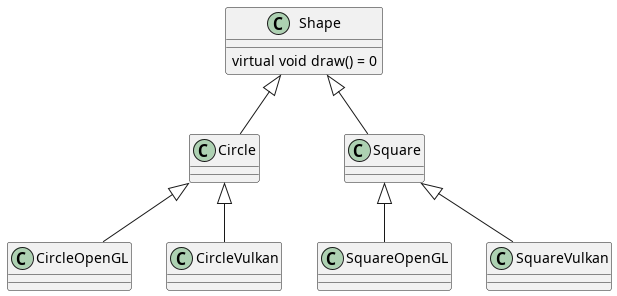
\includegraphics{OldPoly.png}

Результаты такого подхода:

\begin{itemize}
\tightlist
\item
  Очень много наследования
\item
  Нелепые имена классов
\item
  Огромные иерархии классов
\item
  Дублирования кода (DRY)
\item
  Невероятно сложное добавления нового функционала
\item
  Сложность сопровождения кода
\end{itemize}

В попытках справиться с недостатками такого подхода разработчик может
сделать всё ещё хуже.

\hypertarget{ux43fux430ux442ux442ux435ux440ux43dux44b}{%
\section{Паттерны}\label{ux43fux430ux442ux442ux435ux440ux43dux44b}}

Предыдущий подход был наивным, не имеющим возможности жить в больших
проектах.

Рассмотрим более современный подход - использование паттернов.

Паттерн:

\begin{itemize}
\tightlist
\item
  Имеет имя
\item
  Одним лишь своим именем объясняет уже многое
\item
  Нацелен на уменьшение связности
\item
  Предоставляет своего рода абстракцию
\item
  Проверен временем
\end{itemize}

В тот момент, когда мы добавляли в классы фигур уже второй метод
(\texttt{serialize}), этот паттерн уже витал где-то поблизости. И это
паттерн \textbf{\emph{стратегия}}.

Суть паттерна. (\href{refactoring.guru}{Источник})

Стратегия --- это поведенческий паттерн проектирования, который
определяет семейство схожих алгоритмов и помещает каждый из них в
собственный класс, после чего алгоритмы можно взаимозаменять прямо во
время исполнения программы.

Создадим отдельный класс, определяющий поведение при рисовании фигуры:

\begin{Shaded}
\begin{Highlighting}[]
\KeywordTok{class}\NormalTok{ DrawStrategy}\OperatorTok{\{}
    \KeywordTok{virtual} \DataTypeTok{void}\NormalTok{ draw}\OperatorTok{(}\NormalTok{Circle}\OperatorTok{*)} \OperatorTok{=} \DecValTok{0}\OperatorTok{;}
    \KeywordTok{virtual} \DataTypeTok{void}\NormalTok{ draw}\OperatorTok{(}\NormalTok{Square}\OperatorTok{*)} \OperatorTok{=} \DecValTok{0}\OperatorTok{;}
\OperatorTok{\};}
\end{Highlighting}
\end{Shaded}

Теперь мы можем определить несколько разных методов рисования фигур,
унаследовавшись от \texttt{CircleDrawStrategy}:

\begin{Shaded}
\begin{Highlighting}[]
\KeywordTok{class}\NormalTok{ DrawStrategyOpenGL }\OperatorTok{:} \KeywordTok{public}\NormalTok{ DrawStrategy}\OperatorTok{\{}
    \DataTypeTok{void}\NormalTok{ draw}\OperatorTok{(}\NormalTok{Circle}\OperatorTok{*}\NormalTok{ circle}\OperatorTok{)} \KeywordTok{override} \OperatorTok{\{}
        \CommentTok{// do OpenGL stuff}
    \OperatorTok{\}}
    \DataTypeTok{void}\NormalTok{ draw}\OperatorTok{(}\NormalTok{Square}\OperatorTok{*}\NormalTok{ square}\OperatorTok{)} \KeywordTok{override} \OperatorTok{\{}
        \CommentTok{// do OpenGL stuff}
    \OperatorTok{\}}
\OperatorTok{\};}
\KeywordTok{class}\NormalTok{ DrawStrategyVulkan }\OperatorTok{:} \KeywordTok{public}\NormalTok{ DrawStrategy}\OperatorTok{\{}
    \CommentTok{/* аналогично */}
\OperatorTok{\};}
\end{Highlighting}
\end{Shaded}

А в классе \texttt{Circle} теперь добавим поле, хранящее метод его
рисования.

\begin{Shaded}
\begin{Highlighting}[]
\KeywordTok{struct}\NormalTok{ Circle }\OperatorTok{:} \KeywordTok{public}\NormalTok{ Shape }\OperatorTok{\{}
    \BuiltInTok{std::}\NormalTok{unique\_ptr}\OperatorTok{\textless{}}\NormalTok{DrawStrategy}\OperatorTok{\textgreater{}}\NormalTok{ drawStrategy}\OperatorTok{;}
    \KeywordTok{explicit}\NormalTok{ Circle}\OperatorTok{(}\NormalTok{DrawStrategy }\OperatorTok{*}\NormalTok{drawStrategy}\OperatorTok{)} 
        \OperatorTok{:}\NormalTok{ drawStrategy}\OperatorTok{(}\NormalTok{drawStrategy}\OperatorTok{)} \OperatorTok{\{}
        
    \OperatorTok{\}}
    \DataTypeTok{void}\NormalTok{ draw}\OperatorTok{()} \KeywordTok{override} \OperatorTok{\{}
\NormalTok{        drawStrategy}\OperatorTok{{-}\textgreater{}}\NormalTok{draw}\OperatorTok{(}\KeywordTok{this}\OperatorTok{);}
    \OperatorTok{\}}
\OperatorTok{\};}
\end{Highlighting}
\end{Shaded}

Применение:

\begin{Shaded}
\begin{Highlighting}[]
\DataTypeTok{int}\NormalTok{ main}\OperatorTok{()\{}
    \BuiltInTok{std::}\NormalTok{vector}\OperatorTok{\textless{}}\BuiltInTok{std::}\NormalTok{unique\_ptr}\OperatorTok{\textless{}}\NormalTok{Shape}\OperatorTok{\textgreater{}\textgreater{}}\NormalTok{ v}\OperatorTok{;}
\NormalTok{    v}\OperatorTok{.}\NormalTok{emplace\_back}\OperatorTok{(}
            \BuiltInTok{std::}\NormalTok{make\_unique}\OperatorTok{\textless{}}\NormalTok{Circle}\OperatorTok{\textgreater{}(}\BuiltInTok{std::}\NormalTok{make\_unique}\OperatorTok{\textless{}}\NormalTok{DrawStrategyOpenGL}\OperatorTok{\textgreater{}())}
    \OperatorTok{);}
\NormalTok{    v}\OperatorTok{.}\NormalTok{emplace\_back}\OperatorTok{(}
            \BuiltInTok{std::}\NormalTok{make\_unique}\OperatorTok{\textless{}}\NormalTok{Circle}\OperatorTok{\textgreater{}(}\BuiltInTok{std::}\NormalTok{make\_unique}\OperatorTok{\textless{}}\NormalTok{DrawStrategyVulkan}\OperatorTok{\textgreater{}())}
    \OperatorTok{);}
    \ControlFlowTok{for}\OperatorTok{(}\KeywordTok{auto} \OperatorTok{\&}\NormalTok{sh}\OperatorTok{:}\NormalTok{ v}\OperatorTok{)\{}
\NormalTok{        sh}\OperatorTok{{-}\textgreater{}}\NormalTok{draw}\OperatorTok{();}
    \OperatorTok{\}}
\OperatorTok{\}}
\end{Highlighting}
\end{Shaded}

Таким образом мы выделили в отдельный класс метод рисования. В общем
случае - тот метод, который может в разных обстоятельствах меняться.

Теперь, если потребуется добавить поддержку нового графического движка.
то нужно будет всего лишь добавить новый класс, унаследованный от
\texttt{DrawStrategy}. Не придется менять уже существующий код.

Диаграмма:

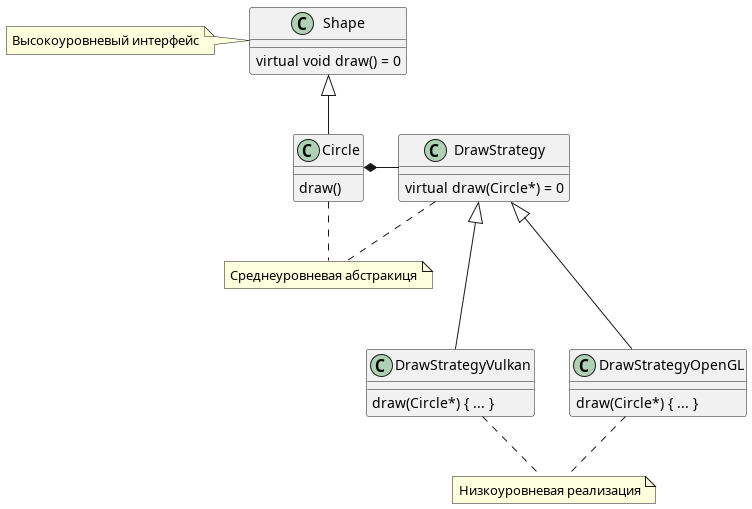
\includegraphics{Strategy.png}

В целом применение паттерна стратегия позволило нам разделить нашу
программу на 3 разных уровня. Вот они, отсортированные по их
абстрактности:

\begin{enumerate}
\def\labelenumi{\arabic{enumi}.}
\tightlist
\item
  Класс \texttt{Shape} - высокоуровневый интерфейс
\item
  Классы \texttt{Circle} и \texttt{Square} - реализации интерфейса
  (средний уровень)
\item
  Абстрактный класс \texttt{DrawStrategy} и его наследники - вынесенное
  в отдельное место поведение (низкоуровневая реализация)
\end{enumerate}

Данный паттерн не ограничивается лишь тем, что наш класс содержит
какой-то внешний объект, содержащий в себе реализацю метода. Стратегии
также распространены и вне мира ООП, например:

\begin{Shaded}
\begin{Highlighting}[]
\BuiltInTok{std::}\NormalTok{vector}\OperatorTok{\textless{}}\DataTypeTok{int}\OperatorTok{\textgreater{}}\NormalTok{ numbers }\OperatorTok{=} \OperatorTok{\{}\DecValTok{1}\OperatorTok{,} \DecValTok{2}\OperatorTok{,} \DecValTok{3}\OperatorTok{,} \DecValTok{4}\OperatorTok{,} \DecValTok{5}\OperatorTok{\};}
\CommentTok{// хотим посчитать сумму чисел}
\BuiltInTok{std::}\NormalTok{accumulate}\OperatorTok{(}
\NormalTok{        numbers}\OperatorTok{.}\NormalTok{cbegin}\OperatorTok{(),}
\NormalTok{        numbers}\OperatorTok{.}\NormalTok{cend}\OperatorTok{(),}
        \DecValTok{0}\OperatorTok{,}
        \BuiltInTok{std::}\NormalTok{plus}\OperatorTok{\{\}} \CommentTok{// \textless{}{-}{-} СТРАТЕГИЯ: "складывать числа"}
\OperatorTok{);}
\CommentTok{// хотим посчитать произведение чисел}
\BuiltInTok{std::}\NormalTok{accumulate}\OperatorTok{(}
\NormalTok{        numbers}\OperatorTok{.}\NormalTok{cbegin}\OperatorTok{(),}
\NormalTok{        numbers}\OperatorTok{.}\NormalTok{cend}\OperatorTok{(),}
        \DecValTok{1}\OperatorTok{,}
        \BuiltInTok{std::}\NormalTok{multiplies}\OperatorTok{\{\}} \CommentTok{// \textless{}{-}{-} СТРАТЕГИЯ: "умножать числа"}
\OperatorTok{);}
\end{Highlighting}
\end{Shaded}

Стратегии в стандартной библиотеке шаблонов:

\begin{Shaded}
\begin{Highlighting}[]
\KeywordTok{template}\OperatorTok{\textless{}}
    \KeywordTok{typename}\NormalTok{ \_Tp}\OperatorTok{,}
    \KeywordTok{typename}\NormalTok{ \_Alloc }\OperatorTok{=} \BuiltInTok{std::}\NormalTok{allocator}\OperatorTok{\textless{}}\NormalTok{\_Tp}\OperatorTok{\textgreater{}}  \CommentTok{// \textless{}{-}{-} СТРАТЕГИЯ. }
                \CommentTok{//Аллокатор определяет, как будет выделяться память}
        \OperatorTok{\textgreater{}}
    \KeywordTok{class}\NormalTok{ vector }\OperatorTok{\{}\CommentTok{/* ... */}\OperatorTok{\};}

\KeywordTok{template}\OperatorTok{\textless{}}
    \KeywordTok{typename}\NormalTok{ \_Value}\OperatorTok{,}
    \KeywordTok{typename}\NormalTok{ \_Hash }\OperatorTok{=}\NormalTok{ hash}\OperatorTok{\textless{}}\NormalTok{\_Value}\OperatorTok{\textgreater{},}       \CommentTok{// \textless{}{-}{-} СТРАТЕГИЯ Хеш функция}
    \KeywordTok{typename}\NormalTok{ \_Pred }\OperatorTok{=}\NormalTok{ equal\_to}\OperatorTok{\textless{}}\NormalTok{\_Value}\OperatorTok{\textgreater{},}   \CommentTok{// \textless{}{-}{-} СТРАТЕГИЯ Как сравнивать ключи}
    \KeywordTok{typename}\NormalTok{ \_Alloc }\OperatorTok{=}\NormalTok{ allocator}\OperatorTok{\textless{}}\NormalTok{\_Value}\OperatorTok{\textgreater{}}  \CommentTok{// \textless{}{-}{-} СТРАТЕГИЯ (см. выше)}
       \OperatorTok{\textgreater{}}
    \KeywordTok{class}\NormalTok{ unordered\_set }\OperatorTok{\{}\CommentTok{/* ... */}\OperatorTok{\};}

\KeywordTok{template} \OperatorTok{\textless{}}
    \KeywordTok{typename}\NormalTok{ \_Tp}\OperatorTok{,} 
    \KeywordTok{typename}\NormalTok{ \_Dp }\OperatorTok{=}\NormalTok{ default\_delete}\OperatorTok{\textless{}}\NormalTok{\_Tp}\OperatorTok{\textgreater{}} \CommentTok{// \textless{}{-}{-} СТРАТЕГИЯ }
                            \CommentTok{// Как освобождать память}
    \OperatorTok{\textgreater{}}
    \KeywordTok{class}\NormalTok{ unique\_ptr}
\end{Highlighting}
\end{Shaded}

Итоги применения паттерна стратегия:

\begin{itemize}
\tightlist
\item
  Вынесение деталей реализации в отдельные классы. (Принцип единственной
  ответственности/Single responsibility principle)
\item
  Создали возможность легкого расширения (Принцип открытости/закрытости.
  OCP)
\item
  Разделили интерфейсы (Interface segregation principle)
\item
  Избавились от дублирования кода (DRY)
\item
  Избавились от глубины иерархии
\item
  Упростили сопровождение кода. Легче понимать, легче писать
\end{itemize}

Но! Минусы:

\begin{itemize}
\tightlist
\item
  Производительность с точки зрения вызовов. При вызове \texttt{draw}
  происходит на самом деле два вызова: \texttt{main} -\textgreater{}
  \texttt{Circle::draw} -\textgreater{}
  \texttt{DrawStrategy::draw(Circle*)}
\item
  Производительность с точки зрения памяти. Множество маленьких
  выделений памяти для стратегий.
\item
  Производительность с точки зрения указателей. Много указателей, мы
  переходим по их адресам.
\item
  Нужно создавать отдельные абстрактные классы-стратегии для другой
  функциональности, например \texttt{SerializeStrategy} для
  сериализации.
\item
  Если отказаться от умных указателей в пользу производительности, то
  придётся вручную управлять временем жизни объектов. См.
  \href{https://youtu.be/rHIkrotSwcc}{Интересная лекция про цену
  абстракций}.
\item
  \texttt{Circle} и \texttt{Square} всё еще знают про то, что их нужно
  как-то рисовать. Они всё еще несут некоторую ответственность за эти
  операции. Что-то в этом чувствуется не так. Операция рисования,
  конечно, зависит от фигуры, которая рисуется в данный момент. Но по
  идее самой фигуре не должно быть дела, рисуют ли её или делают что-то
  другое. Это слегка размывает абстракцию фигуры.
\end{itemize}

Существует решение лучше!

\hypertarget{ux434ux432ux438ux433ux430ux435ux43cux441ux44f-ux43a-type-erasure}{%
\section{Двигаемся к Type
Erasure}\label{ux434ux432ux438ux433ux430ux435ux43cux441ux44f-ux43a-type-erasure}}

Вы уже могли слышать что-то про стирание типа, поэтому уточню:

\begin{itemize}
\tightlist
\item
  Это НЕ про

  \begin{itemize}
  \tightlist
  \item
    это не про \texttt{void*}
  \item
    это не про указатели на базовый класс
  \item
    это не про \texttt{std::variant}. \texttt{std::variant} основан на
    фиксированном наборе типов и предоставляет открытый набор операций
    над ними. Мы же пытаемся достигнуть обратного - открытого для
    расширения набора типов и фиксированного набора операций над ними.
  \end{itemize}
\item
  Это про

  \begin{itemize}
  \tightlist
  \item
    Шаблонный конструктор
  \item
    Интерфейс без единого слова \texttt{virtual}
  \item
    Смесь паттернов External Poymorphism, Bridge, Prototype
  \end{itemize}
\end{itemize}

Посмотрим на класс \texttt{Circle}, ещё не испорченный разными не
относящимися к фигурам методами, а также наследованием:

\begin{Shaded}
\begin{Highlighting}[]
\KeywordTok{class}\NormalTok{ Circle }\OperatorTok{\{}
\KeywordTok{public}\OperatorTok{:}
    \KeywordTok{explicit}\NormalTok{ Circle}\OperatorTok{(}\DataTypeTok{double}\NormalTok{ r}\OperatorTok{)}
            \OperatorTok{:}\NormalTok{ radius}\OperatorTok{(}\NormalTok{r}\OperatorTok{)} \OperatorTok{\{\}}

    \DataTypeTok{double}\NormalTok{ getRadius}\OperatorTok{()} \AttributeTok{const} \OperatorTok{\{}
        \ControlFlowTok{return}\NormalTok{ radius}\OperatorTok{;}
    \OperatorTok{\}}

    \DataTypeTok{void}\NormalTok{ setRadius}\OperatorTok{(}\DataTypeTok{double}\NormalTok{ r}\OperatorTok{)} \OperatorTok{\{}
\NormalTok{        radius }\OperatorTok{=}\NormalTok{ r}\OperatorTok{;}
    \OperatorTok{\}}

\KeywordTok{private}\OperatorTok{:}
    \DataTypeTok{double}\NormalTok{ radius}\OperatorTok{;}
    \CommentTok{// тут могут быть еще полезные данные}
    \CommentTok{// координаты центра например}
\OperatorTok{\};}
\end{Highlighting}
\end{Shaded}

И аналогично может быть определён класс \texttt{Square}.

\begin{itemize}
\tightlist
\item
  Этим классам не нужен базовый класс
\item
  Им не нужно знать друг о друге
\item
  Они не должны забатиться о том, что с ними можно сделать
\end{itemize}

Это очень удобно. Такими классами максимально просто пользоваться. У них
нет никаких зависимостей. И это главное - мы их больше никогда не
изменим!

Теперь перейдем к решению проблемы их рисования.

\hypertarget{ux43fux430ux442ux442ux435ux440ux43d-external-polymorphism}{%
\subsection{Паттерн External
Polymorphism}\label{ux43fux430ux442ux442ux435ux440ux43d-external-polymorphism}}

Описание задачи этого паттерна из исходного документа, описывающего его:

\emph{Allow classes that are not related by inheritance and/or have no
virtual methods to be treated polymorphically.}

И мой вольный перевод:

\emph{Дать возможность классам, не связанным наследованием и/или не
имеющим виртуальных методов, быть обработанными так, как будто они
полиморфные.}

Посмотрим на данный код и разберем, что к чему

\begin{Shaded}
\begin{Highlighting}[]
\KeywordTok{struct}\NormalTok{ ShapeConcept }\OperatorTok{\{}
    \KeywordTok{virtual} \OperatorTok{\textasciitilde{}}\NormalTok{ShapeConcept}\OperatorTok{()} \OperatorTok{=} \ControlFlowTok{default}\OperatorTok{;}
\OperatorTok{\};}

\KeywordTok{template}\OperatorTok{\textless{}}\KeywordTok{typename}\NormalTok{ T}\OperatorTok{\textgreater{}}
\KeywordTok{struct}\NormalTok{ ShapeModel }\OperatorTok{:} \KeywordTok{public}\NormalTok{ ShapeConcept }\OperatorTok{\{}
\NormalTok{    T object}\OperatorTok{;}

    \KeywordTok{explicit}\NormalTok{ ShapeModel}\OperatorTok{(}\NormalTok{T }\OperatorTok{\&\&}\NormalTok{shape}\OperatorTok{)} \OperatorTok{:}\NormalTok{ object}\OperatorTok{(}\BuiltInTok{std::}\NormalTok{move}\OperatorTok{(}\NormalTok{shape}\OperatorTok{))} \OperatorTok{\{\}}

    \KeywordTok{explicit}\NormalTok{ ShapeModel}\OperatorTok{(}\AttributeTok{const}\NormalTok{ T }\OperatorTok{\&}\NormalTok{shape}\OperatorTok{)} \OperatorTok{:}\NormalTok{ object}\OperatorTok{(}\NormalTok{shape}\OperatorTok{)} \OperatorTok{\{\}}
\OperatorTok{\};}
\end{Highlighting}
\end{Shaded}

Чуть позже станет ясно, почему здесь написано \texttt{struct}, а не
\texttt{class}. Конструктор \texttt{ShapeModel} принимает объект любого
класса и сохраняет его в своё поле. Этим классом может быть
\texttt{Circle} или \texttt{Square}, или любая другая фигура, которую мы
создадим.

В то же время \texttt{ShapeModel} наследуется от \texttt{ShapeConcept},
чуть позже станет ясно, почему.

Теперь в \texttt{ShapeConcept} добавим все функции-операции над
фигурами, которые могут быть нужны нам (оставлю в будущем только
\texttt{draw} для краткости).

\begin{Shaded}
\begin{Highlighting}[]
\KeywordTok{struct}\NormalTok{ ShapeConcept }\OperatorTok{\{}
    \KeywordTok{virtual} \OperatorTok{\textasciitilde{}}\NormalTok{ShapeConcept}\OperatorTok{()} \OperatorTok{=} \ControlFlowTok{default}\OperatorTok{;}
    \KeywordTok{virtual} \DataTypeTok{void}\NormalTok{ draw}\OperatorTok{()} \AttributeTok{const} \OperatorTok{=} \DecValTok{0}\OperatorTok{;}
    \CommentTok{// ...}
\OperatorTok{\};}
\end{Highlighting}
\end{Shaded}

И особенным образом дадим определение этим функциям в производном классе
\texttt{ShapeModel}:

\begin{Shaded}
\begin{Highlighting}[]
\KeywordTok{template}\OperatorTok{\textless{}}\KeywordTok{typename}\NormalTok{ T}\OperatorTok{\textgreater{}}
\KeywordTok{struct}\NormalTok{ ShapeModel }\OperatorTok{:} \KeywordTok{public}\NormalTok{ ShapeConcept }\OperatorTok{\{}
\NormalTok{    T object}\OperatorTok{;}

    \KeywordTok{explicit}\NormalTok{ ShapeModel}\OperatorTok{(}\NormalTok{T }\OperatorTok{\&\&}\NormalTok{shape}\OperatorTok{)} \OperatorTok{:}\NormalTok{ object}\OperatorTok{(}\BuiltInTok{std::}\NormalTok{move}\OperatorTok{(}\NormalTok{shape}\OperatorTok{))} \OperatorTok{\{\}}

    \KeywordTok{explicit}\NormalTok{ ShapeModel}\OperatorTok{(}\AttributeTok{const}\NormalTok{ T }\OperatorTok{\&}\NormalTok{shape}\OperatorTok{)} \OperatorTok{:}\NormalTok{ object}\OperatorTok{(}\NormalTok{shape}\OperatorTok{)} \OperatorTok{\{\}}

    \DataTypeTok{void}\NormalTok{ draw}\OperatorTok{()} \AttributeTok{const} \KeywordTok{override} \OperatorTok{\{}
\NormalTok{        draw}\OperatorTok{(}\NormalTok{object}\OperatorTok{);} \CommentTok{// Что за функция draw? См. после кода.}
    \OperatorTok{\}}
\OperatorTok{\};}
\end{Highlighting}
\end{Shaded}

Что же за вызов функции \texttt{draw(object)}? Когда мы пишем такое, мы
утверждаем, что где-то вне классов, только что созданных нами,
существует функция \texttt{draw}, которая в качестве аргумента сможет
принять \texttt{object} типа \texttt{T}.

Например: \texttt{void\ draw(const\ Circle\ \&c)\ \{\ ...\ \}}

Это уже наложило ограничения на то, какие типы могут быть подставлены
вместо \texttt{T} во время инстанциации шаблона \texttt{ShapeModel}. А
именно: для этих типов обязательно должна существовать функция,
принимающая их в качестве аргумента.

\texttt{ShapeModel} наследуется от \texttt{ShapeConcept}. Таким образом,
с помощью задания чисто виртуальных функций в классе
\texttt{ShapeConcept} мы говорим, какие функции-обработчики должны
обязательно существовать для объектов, которые мы будем в будущем
хранить внутри \texttt{ShapeModel}.

В этом и заключается паттерн External Polymorphism.

\begin{itemize}
\tightlist
\item
  Мы извлекли полиморфную часть классов иерархии(которая теперь уже и не
  нужна) в отдельное место
\item
  Мы всё еще можем строго задавать функции-обработчики наших классов
\item
  Всё еще могут существовать абстрактные классы (для которых нет полного
  набора функций-обработчиков)
\end{itemize}

Диаграмма для паттерна External Polymorphism.

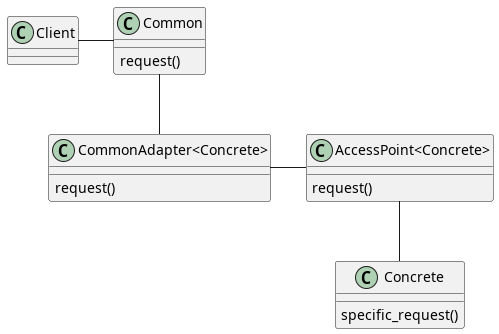
\includegraphics{EP.png}

В итоге данный паттерн:

\begin{itemize}
\tightlist
\item
  Позволяет обрабатывать \textbf{\emph{любой}} объект так, как будто он
  полиморфный. Можно даже создать видимость полиморфизма для
  фундаментальных типов (например \texttt{int})
\item
  Позволяет вынести детали реализации из класса
\item
  Позволяет классам не заботиться (и даже знать) о тех операциях,
  которые над ними совершаются
\item
  Открывает возможность лёгкого расширения функциональности
\end{itemize}

Покажу пример работы:

\begin{Shaded}
\begin{Highlighting}[]
\KeywordTok{class}\NormalTok{ Circle }\OperatorTok{\{} \CommentTok{/* см. выше */} \OperatorTok{\};}
\KeywordTok{struct}\NormalTok{ ShapeConcept }\OperatorTok{\{} \CommentTok{/* см. выше */} \OperatorTok{\};}

\KeywordTok{template}\OperatorTok{\textless{}}\KeywordTok{typename}\NormalTok{ T}\OperatorTok{\textgreater{}}
\KeywordTok{struct}\NormalTok{ ShapeModel }\OperatorTok{:} \KeywordTok{public}\NormalTok{ ShapeConcept }\OperatorTok{\{} \CommentTok{/* см. выше */} \OperatorTok{\};}

\CommentTok{// Определим функцию, которая умеет рисовать круг}
\DataTypeTok{void}\NormalTok{ draw}\OperatorTok{(}\AttributeTok{const}\NormalTok{ Circle }\OperatorTok{\&}\NormalTok{s}\OperatorTok{)} \OperatorTok{\{}
  \BuiltInTok{std::}\NormalTok{cout}\OperatorTok{ \textless{}\textless{}} \StringTok{"I am Circle with radius = "} \OperatorTok{\textless{}\textless{}} 
\NormalTok{        s}\OperatorTok{.}\NormalTok{getRadius}\OperatorTok{()} \OperatorTok{\textless{}\textless{}} \BuiltInTok{std::}\NormalTok{endl}\OperatorTok{;}
\OperatorTok{\}}
\CommentTok{// Теперь класс Circle отвечает требованиям ShapeConcept}
\DataTypeTok{int}\NormalTok{ main}\OperatorTok{()\{}
    \BuiltInTok{std::}\NormalTok{vector}\OperatorTok{\textless{}}\BuiltInTok{std::}\NormalTok{unique\_ptr}\OperatorTok{\textless{}}\NormalTok{ShapeConcept}\OperatorTok{\textgreater{}\textgreater{}}\NormalTok{ v}\OperatorTok{;}
\NormalTok{    v}\OperatorTok{.}\NormalTok{emplace\_back}\OperatorTok{(}\BuiltInTok{std::}\NormalTok{make\_unique}\OperatorTok{\textless{}}\NormalTok{ShapeModel}\OperatorTok{\textless{}}\NormalTok{Circle}\OperatorTok{\textgreater{}\textgreater{}\{}\FloatTok{3.0}\OperatorTok{\});}
\NormalTok{    v}\OperatorTok{.}\NormalTok{emplace\_back}\OperatorTok{(}\BuiltInTok{std::}\NormalTok{make\_unique}\OperatorTok{\textless{}}\NormalTok{ShapeModel}\OperatorTok{\textless{}}\NormalTok{Circle}\OperatorTok{\textgreater{}\textgreater{}\{}\FloatTok{4.0}\OperatorTok{\});}
\NormalTok{    v}\OperatorTok{.}\NormalTok{emplace\_back}\OperatorTok{(}\BuiltInTok{std::}\NormalTok{make\_unique}\OperatorTok{\textless{}}\NormalTok{ShapeModel}\OperatorTok{\textless{}}\NormalTok{Circle}\OperatorTok{\textgreater{}\textgreater{}\{}\FloatTok{5.0}\OperatorTok{\});}
    \ControlFlowTok{for}\OperatorTok{(}\KeywordTok{auto} \OperatorTok{*}\NormalTok{shape}\OperatorTok{:}\NormalTok{ v}\OperatorTok{)\{}
\NormalTok{        shape}\OperatorTok{{-}\textgreater{}}\NormalTok{draw}\OperatorTok{();}
    \OperatorTok{\}}
  
  \CommentTok{// int не отвечает требованиям ShapeConcept}
  \CommentTok{// следующий код не скомпилируется}
  \CommentTok{// ошибка при инстанциации класса ShapeModel\textless{}int\textgreater{}}
  \CommentTok{// так как нет функци draw(int)}
\NormalTok{  ShapeModel text}\OperatorTok{(}\DecValTok{123}\OperatorTok{);} 
\OperatorTok{\}}
\end{Highlighting}
\end{Shaded}

И\ldots{} Ура! Это работает! Но.

Из оригинального документа, описывающего данный паттерн есть ещё один
пример. Допустим, мы работаем с несколькими библиотеками и хотим
написать сериализацию для объектов из этих библиотек. Взять и создать
для них общий базовый класс не представляется возможным. С помощью
данного паттерна мы можем решить эту проблему.

Создаем класс \texttt{SerializableConcept}, который описывает, какие
внешние функции должны существовать (\texttt{serialize} в данном
случае). От этого класса наследуем класс \texttt{SerializableModel}
(аналогично \texttt{ShapeModel}). И получаем возможность создать
\texttt{SerializableModel} над любым классом, для которого существует
функция \texttt{serialize}, принимающая этот класс как аргумент. И,
соответственно, теперь мы можем сериализовать любой класс.

Подведём итоги применения паттерна External Polymorphism:

\begin{itemize}
\tightlist
\item
  Много указателей
\item
  Много \texttt{std::make\_unique}
\item
  И много других вещей, которые мы не хотим делать вручную
\end{itemize}

Давайте улучшим этот паттерн, чтобы избавиться от данных проблем.

\hypertarget{type-erasure}{%
\section{Type Erasure}\label{type-erasure}}

Возьмём и обернем \texttt{ShapeConcept} и \texttt{ShapeModel} в класс
\texttt{Shape}, в его секцию \texttt{private} (становится понятно, зачем
было объявлять их \texttt{struct} - теперь они всё равно спрятаны).

\begin{Shaded}
\begin{Highlighting}[]
\KeywordTok{class}\NormalTok{ Shape }\OperatorTok{\{}
\KeywordTok{private}\OperatorTok{:}
    \KeywordTok{struct}\NormalTok{ ShapeConcept }\OperatorTok{\{} \CommentTok{/* см. выше */} \OperatorTok{\};}

    \KeywordTok{template}\OperatorTok{\textless{}}\KeywordTok{typename}\NormalTok{ T}\OperatorTok{\textgreater{}}
    \KeywordTok{struct}\NormalTok{ ShapeModel }\OperatorTok{:} \KeywordTok{public}\NormalTok{ ShapeConcept }\OperatorTok{\{} \CommentTok{/* см. выше */} \OperatorTok{\};}
\OperatorTok{\};}
\end{Highlighting}
\end{Shaded}

Таким образом мы прячем эти относительно искусственные два класса с не
очень говорящими именами внутрь уже довольно очевидной оболочки.

Теперь предоставим пользователю возможность создать любую фигуру.
Добавим в класс \texttt{Shape} поле, хранящее конкретную фигуру и
шаблонный конструктор:

\begin{Shaded}
\begin{Highlighting}[]
\KeywordTok{class}\NormalTok{ Shape }\OperatorTok{\{}
\KeywordTok{private}\OperatorTok{:}
    \KeywordTok{struct}\NormalTok{ ShapeConcept }\OperatorTok{\{} \CommentTok{/* см. выше */} \OperatorTok{\};}

    \KeywordTok{template}\OperatorTok{\textless{}}\KeywordTok{typename}\NormalTok{ T}\OperatorTok{\textgreater{}}
    \KeywordTok{struct}\NormalTok{ ShapeModel }\OperatorTok{:} \KeywordTok{public}\NormalTok{ ShapeConcept }\OperatorTok{\{} \CommentTok{/* см. выше */} \OperatorTok{\};}
    
    \BuiltInTok{std::}\NormalTok{unique\_ptr}\OperatorTok{\textless{}}\NormalTok{ShapeConcept}\OperatorTok{\textgreater{}}\NormalTok{ shapePtr}\OperatorTok{;} \CommentTok{// новое поле}
\KeywordTok{public}\OperatorTok{:}
    \KeywordTok{template}\OperatorTok{\textless{}}\KeywordTok{typename}\NormalTok{ T}\OperatorTok{\textgreater{}}
    \KeywordTok{explicit}\NormalTok{ Shape}\OperatorTok{(}\NormalTok{T }\OperatorTok{\&\&}\NormalTok{shape}\OperatorTok{)} 
        \OperatorTok{:}\NormalTok{ shapePtr}\OperatorTok{(}\KeywordTok{new}\NormalTok{ ShapeModel}\OperatorTok{\textless{}}\NormalTok{T}\OperatorTok{\textgreater{}(}\BuiltInTok{std::}\NormalTok{forward}\OperatorTok{(}\NormalTok{shape}\OperatorTok{)))} \OperatorTok{\{\}}
\OperatorTok{\};}
\end{Highlighting}
\end{Shaded}

А теперь присмотритесь. Что делает этот новый конструктор? Он создает
для переданного объекта соответсвующую ему \texttt{ShapeModel}.
Заметьте, новое поле имеет тип
\texttt{std::unique\_ptr\textless{}ShapeConcept\textgreater{}} и
конструктор сохраняет в него указатель на ShapeModel. А теперь посмотрим
на то, что происходит с типами во время всех этих действий:

\begin{enumerate}
\def\labelenumi{\arabic{enumi}.}
\tightlist
\item
  Объект передан в конструктор \texttt{Shape} - тип известен
  (\texttt{T})
\item
  Создан объект класса \texttt{ShapeModel\textless{}T\textgreater{}} -
  тип исходного объекта всё еще здесь
\item
  Указатель на \texttt{ShapeModel\textless{}T\textgreater{}} сохранен
  внутри указателя на \texttt{ShapeConcept}. Так можно сделать, ведь они
  связаны наследованием. Но! Указатель на \texttt{ShapeConcept} уже не
  содержит в себе типа, который лежит внутри него. На этом шаге и
  произошло ``стирание типа''. Отсюда и название данного паттерна.
\end{enumerate}

Но несмотря на то, что тип кажется утерянным, мы всё еще можем
пользоваться объектом, который только что сохранили. Всё, что нужно для
его обработки уже написано в классах \texttt{ShapeConcept} и
\texttt{ShapeModel}. Нужна лишь внешняя функция-обработчик.

Этот шаг с созданием шаблонного конструктора \texttt{Shape} и есть
проявляение паттерна Bridge.

Для справки (wikipedia):

\begin{itemize}
\tightlist
\item
  Мост - структурный шаблон проектирования, используемый в
  проектировании программного обеспечения чтобы «разделять абстракцию и
  реализацию так, чтобы они могли изменяться независимо»
\end{itemize}

Теперь мы можем создать сколько нам угодно классов для разных фигур,
создать перегрузки функции \texttt{draw}, способные принимать объекты их
типов в качестве аргументов. А красота в том, что компилятор
инстанциирует нужные шаблоны и предоставит нам возможность пользоваться
ими, как полиморфными! Нам самим не нужно писать этот код.

И последнее, что нужно для пользования классом \texttt{Shape}. Все еще
нет возможности нарисовать сохраненную фигуру. Для решения этой проблемы
создадим функцию:

\begin{Shaded}
\begin{Highlighting}[]
\KeywordTok{class}\NormalTok{ Shape }\OperatorTok{\{}
\KeywordTok{private}\OperatorTok{:}
    \CommentTok{/* см. выше */}
\KeywordTok{public}\OperatorTok{:}
    \CommentTok{/* конструктор */}
    
    \KeywordTok{friend} \DataTypeTok{void}\NormalTok{ draw}\OperatorTok{(}\AttributeTok{const}\NormalTok{ Shape }\OperatorTok{\&}\NormalTok{shape}\OperatorTok{)} \OperatorTok{\{}
\NormalTok{        shape}\OperatorTok{.}\NormalTok{shapePtr}\OperatorTok{{-}\textgreater{}}\NormalTok{draw}\OperatorTok{();}
        \CommentTok{// shape                    {-}  Тип Shape}
        \CommentTok{// shape.ShapePtr           {-}  Тип ShapeConcept}
        \CommentTok{// shape.ShapePtr{-}\textgreater{}draw()   {-}\textgreater{} Вызов ShapeModel::draw()}
        \CommentTok{// Внутри реализации}
        \CommentTok{// Вызов ShapeModel::draw() {-}\textgreater{} Вызов draw(T)}
    \OperatorTok{\}}
\OperatorTok{\};}
\end{Highlighting}
\end{Shaded}

Новая функция должна быть объявлена с словом \texttt{friend}, чтобы она
могла внутри себя обратиться к полю \texttt{shapePtr} класса
\texttt{Shape}.

Пример применения:

\begin{Shaded}
\begin{Highlighting}[]
\DataTypeTok{int}\NormalTok{ main}\OperatorTok{()\{}
\NormalTok{    Shape circle}\OperatorTok{(}\NormalTok{Circle}\OperatorTok{\{}\FloatTok{3.14}\OperatorTok{\});}
\NormalTok{    draw}\OperatorTok{(}\NormalTok{circle}\OperatorTok{);} \CommentTok{// красиво!}
\OperatorTok{\}}
\end{Highlighting}
\end{Shaded}

Теперь этим можно пользоваться, рисовать разные фигуры. Но, скорее
всего, в скором времени возникнет проблема. Как копировать объекты
класса \texttt{Shape}? Ведь этот класс не знает тип объекта, который он
хранит внутри себя.

С решением этой проблемы поможет паттерн Прототип.

Суть паттерна. Прототип --- это порождающий паттерн проектирования,
который позволяет копировать объекты, не вдаваясь в подробности их
реализации.

Просто добавим новый чисто виртуальный метод \texttt{clone} в
\texttt{ShapeConcept}:

\begin{Shaded}
\begin{Highlighting}[]
\KeywordTok{struct}\NormalTok{ ShapeConcept }\OperatorTok{\{}
    \KeywordTok{virtual} \OperatorTok{\textasciitilde{}}\NormalTok{ShapeConcept}\OperatorTok{()} \OperatorTok{=} \ControlFlowTok{default}\OperatorTok{;}
    \KeywordTok{virtual} \BuiltInTok{std::}\NormalTok{unique\_ptr}\OperatorTok{\textless{}}\NormalTok{ShapeConcept}\OperatorTok{\textgreater{}}\NormalTok{ clone}\OperatorTok{()} \AttributeTok{const} \OperatorTok{=} \DecValTok{0}\OperatorTok{;}
    \KeywordTok{virtual} \DataTypeTok{void}\NormalTok{ draw}\OperatorTok{()} \AttributeTok{const} \OperatorTok{=} \DecValTok{0}\OperatorTok{;}
    \CommentTok{// ...}
\OperatorTok{\};}
\end{Highlighting}
\end{Shaded}

Теперь этот новый метод отвечает за копирование (клонирование) объектов.

Дадим этому методу определение в \texttt{ShapeModel}:

\begin{Shaded}
\begin{Highlighting}[]

\KeywordTok{template}\OperatorTok{\textless{}}\KeywordTok{typename}\NormalTok{ T}\OperatorTok{\textgreater{}}
\KeywordTok{struct}\NormalTok{ ShapeModel }\OperatorTok{:}
\KeywordTok{public}\NormalTok{ ShapeConcept }\OperatorTok{\{}
\CommentTok{/* всё остальное */}

\BuiltInTok{std::}\NormalTok{unique\_ptr}\OperatorTok{\textless{}}\NormalTok{ShapeConcept}\OperatorTok{\textgreater{}}\NormalTok{ clone}\OperatorTok{()} \AttributeTok{const} \KeywordTok{override} \OperatorTok{\{}
\ControlFlowTok{return} \BuiltInTok{std::}\NormalTok{make\_unique}\OperatorTok{\textless{}}\NormalTok{ShapeModel}\OperatorTok{\textgreater{}(*}\KeywordTok{this}\OperatorTok{);}
\OperatorTok{\}}
\OperatorTok{\};}
\end{Highlighting}
\end{Shaded}

Конечно же, дадим пользователю возможность использовать этот метод,
добавим соотвествующую функцию в \texttt{Shape}:

\begin{Shaded}
\begin{Highlighting}[]
\KeywordTok{class}\NormalTok{ Shape }\OperatorTok{\{}
\KeywordTok{private}\OperatorTok{:}
    \CommentTok{/* см. выше */}
    \BuiltInTok{std::}\NormalTok{unique\_ptr}\OperatorTok{\textless{}}\NormalTok{ShapeConcept}\OperatorTok{\textgreater{}}\NormalTok{ shapePtr}\OperatorTok{;}
\KeywordTok{public}\OperatorTok{:}
    \CommentTok{/* всё остальное */}
    
\NormalTok{    Shape}\OperatorTok{(}\AttributeTok{const}\NormalTok{ Shape}\OperatorTok{\&}\NormalTok{ other}\OperatorTok{)} 
        \OperatorTok{:}\NormalTok{ shapePtr}\OperatorTok{(}\NormalTok{other}\OperatorTok{.}\NormalTok{shapePtr}\OperatorTok{{-}\textgreater{}}\NormalTok{clone}\OperatorTok{();)} \OperatorTok{\{\}}
\OperatorTok{\};}
\end{Highlighting}
\end{Shaded}

Теперь можно написать так:

\begin{Shaded}
\begin{Highlighting}[]
\DataTypeTok{int}\NormalTok{ main}\OperatorTok{()\{}
\NormalTok{    Shape circle}\OperatorTok{(}\NormalTok{Circle}\OperatorTok{\{}\FloatTok{3.14}\OperatorTok{\});}
    \KeywordTok{auto}\NormalTok{ circle\_copy }\OperatorTok{=}\NormalTok{ circle}\OperatorTok{;}
\NormalTok{    draw}\OperatorTok{(}\NormalTok{circle\_copy}\OperatorTok{);}
\OperatorTok{\}}
\end{Highlighting}
\end{Shaded}

Анализ данного решения:

\begin{enumerate}
\def\labelenumi{\arabic{enumi}.}
\tightlist
\item
  \texttt{Shape} - высокоуровневая абстракция ``контейнера'' для фигур,
  который позволяет хранить в себе только те фигуры, которые
  соответствуют требованиям ShapeConcept.
\item
  \texttt{Circle}, \texttt{Square} и др. - содержат только нужную
  информацию. Не знают о классе \texttt{Shape}. Не знают об операциях
  над ними. Не связаны полиморфизмом. Среднеуровневая абстракции.
\item
  Функции \texttt{draw}, \texttt{serialize} и др. Делают некие операции
  над нужными фигурами - низкоуровневая абстракция.
\item
  \texttt{ShapeModel} - хранит в себе конкретную фигуру, связывает
  \texttt{Shape} с конкретными функциями-обработчиками фигур (Мост).
  Сгенерирован компилятором.
\end{enumerate}

Что мы получили:

\begin{itemize}
\tightlist
\item
  Извлекли детали реализации
\item
  Предоставили возможность лёгкого расширения функциональности
\item
  Разделение интерфейсов
\item
  Отсутствие дублирования кода
\item
  Классы, с которыми мы работаем, больше не отвечают за операции,
  которые производятся над ними. Они не обязаны знать о них.
\item
  Нет больших иерархий наследования.
\item
  Нет указателей (для пользователя)
\item
  Нет ручного управления памятью (для пользователя)
\item
  Улучшили производительность
\item
  И это всё в \texttt{private} секции нового класса \texttt{Shape}!
\end{itemize}

В итоге. Что такое Type Erasure?

\begin{itemize}
\tightlist
\item
  Шаблонный конструктор
\item
  Полностью НЕвиртуальный интерфейс (спасибо, External Polymorphism)
\item
  External Polymorphism + Bridge + Prototype
\item
  Очень элегантный современный паттерн :)
\end{itemize}

Что Type Erasure позволяет сделать?

\begin{itemize}
\tightlist
\item
  Избавиться от зависимостей
\item
  Избавиться от указателей
\item
  Улучшить производительность
\item
  Улучшить читабельность и ``понимательность'' кода
\item
  Упростить сопровождение кода
\end{itemize}

Диаграмма паттерна Type Erasure:

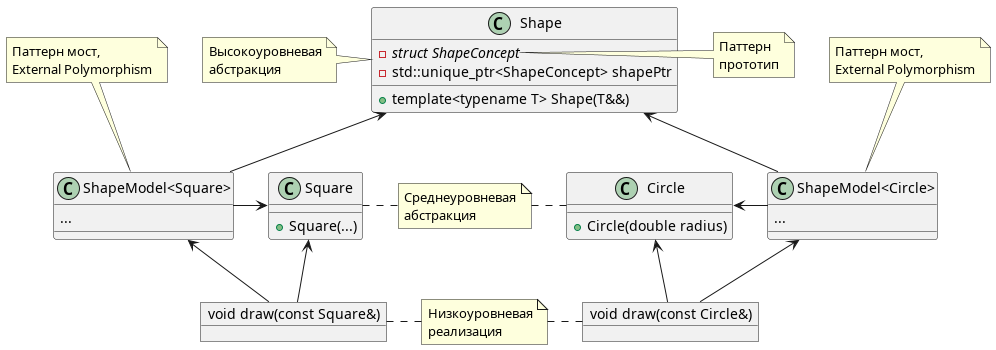
\includegraphics{TE.png}

\hypertarget{ux43fux43eux43bux43dux44bux439-ux43aux43eux434}{%
\section{Полный
код}\label{ux43fux43eux43bux43dux44bux439-ux43aux43eux434}}

\begin{Shaded}
\begin{Highlighting}[]
\PreprocessorTok{\#include }\ImportTok{\textless{}iostream\textgreater{}}
\PreprocessorTok{\#include }\ImportTok{\textless{}memory\textgreater{}}
\PreprocessorTok{\#include }\ImportTok{\textless{}vector\textgreater{}}

\KeywordTok{class}\NormalTok{ Shape }\OperatorTok{\{}
\KeywordTok{private}\OperatorTok{:}
    \KeywordTok{struct}\NormalTok{ ShapeConcept }\OperatorTok{\{}
        \KeywordTok{virtual} \DataTypeTok{void}\NormalTok{ drawCall}\OperatorTok{()} \AttributeTok{const} \OperatorTok{=} \DecValTok{0}\OperatorTok{;}

        \KeywordTok{virtual} \BuiltInTok{std::}\NormalTok{unique\_ptr}\OperatorTok{\textless{}}\NormalTok{ShapeConcept}\OperatorTok{\textgreater{}}\NormalTok{ clone}\OperatorTok{()} \AttributeTok{const} \OperatorTok{=} \DecValTok{0}\OperatorTok{;}

        \KeywordTok{virtual} \OperatorTok{\textasciitilde{}}\NormalTok{ShapeConcept}\OperatorTok{()} \OperatorTok{=} \ControlFlowTok{default}\OperatorTok{;}
    \OperatorTok{\};}

    \KeywordTok{template}\OperatorTok{\textless{}}\KeywordTok{typename}\NormalTok{ T}\OperatorTok{\textgreater{}}
    \KeywordTok{struct}\NormalTok{ ShapeModel }\OperatorTok{:} \KeywordTok{public}\NormalTok{ ShapeConcept }\OperatorTok{\{}
\NormalTok{        T shape\_instance}\OperatorTok{;}

        \KeywordTok{explicit}\NormalTok{ ShapeModel}\OperatorTok{(}\NormalTok{T }\OperatorTok{\&\&}\NormalTok{shape}\OperatorTok{)} \OperatorTok{:}\NormalTok{ shape\_instance}\OperatorTok{(}\BuiltInTok{std::}\NormalTok{move}\OperatorTok{(}\NormalTok{shape}\OperatorTok{))} \OperatorTok{\{\}}

        \KeywordTok{explicit}\NormalTok{ ShapeModel}\OperatorTok{(}\AttributeTok{const}\NormalTok{ T }\OperatorTok{\&}\NormalTok{shape}\OperatorTok{)} \OperatorTok{:}\NormalTok{ shape\_instance}\OperatorTok{(}\NormalTok{shape}\OperatorTok{)} \OperatorTok{\{\}}

        \OperatorTok{[[}\AttributeTok{nodiscard}\OperatorTok{]]} \BuiltInTok{std::}\NormalTok{unique\_ptr}\OperatorTok{\textless{}}\NormalTok{ShapeConcept}\OperatorTok{\textgreater{}}\NormalTok{ clone}\OperatorTok{()} \AttributeTok{const} \KeywordTok{override} \OperatorTok{\{}
            \ControlFlowTok{return} \BuiltInTok{std::}\NormalTok{make\_unique}\OperatorTok{\textless{}}\NormalTok{ShapeModel}\OperatorTok{\textgreater{}(*}\KeywordTok{this}\OperatorTok{);}
        \OperatorTok{\}}

        \DataTypeTok{void}\NormalTok{ drawCall}\OperatorTok{()} \AttributeTok{const} \KeywordTok{override} \OperatorTok{\{}
\NormalTok{            draw}\OperatorTok{(}\NormalTok{shape\_instance}\OperatorTok{);}
        \OperatorTok{\}}
    \OperatorTok{\};}

    \BuiltInTok{std::}\NormalTok{unique\_ptr}\OperatorTok{\textless{}}\NormalTok{ShapeConcept}\OperatorTok{\textgreater{}}\NormalTok{ shapePtr}\OperatorTok{;}
\KeywordTok{public}\OperatorTok{:}
    \KeywordTok{template}\OperatorTok{\textless{}}\KeywordTok{typename}\NormalTok{ T}\OperatorTok{\textgreater{}}
    \KeywordTok{explicit}\NormalTok{ Shape}\OperatorTok{(}\NormalTok{T }\OperatorTok{\&\&}\NormalTok{shape}\OperatorTok{)} 
        \OperatorTok{:}\NormalTok{ shapePtr}\OperatorTok{(}\KeywordTok{new}\NormalTok{ ShapeModel}\OperatorTok{\textless{}}\NormalTok{T}\OperatorTok{\textgreater{}(}\BuiltInTok{std::}\NormalTok{forward}\OperatorTok{(}\NormalTok{shape}\OperatorTok{)))} \OperatorTok{\{\}}

    \KeywordTok{friend} \DataTypeTok{void}\NormalTok{ draw}\OperatorTok{(}\AttributeTok{const}\NormalTok{ Shape }\OperatorTok{\&}\NormalTok{shape}\OperatorTok{)} \OperatorTok{\{}
\NormalTok{        shape}\OperatorTok{.}\NormalTok{shapePtr}\OperatorTok{{-}\textgreater{}}\NormalTok{drawCall}\OperatorTok{();}
    \OperatorTok{\}}

\NormalTok{    Shape}\OperatorTok{(}\AttributeTok{const}\NormalTok{ Shape }\OperatorTok{\&}\NormalTok{other}\OperatorTok{)} \OperatorTok{:}\NormalTok{ shapePtr}\OperatorTok{(}\NormalTok{other}\OperatorTok{.}\NormalTok{shapePtr}\OperatorTok{{-}\textgreater{}}\NormalTok{clone}\OperatorTok{())} \OperatorTok{\{}
    \OperatorTok{\}}
\OperatorTok{\};}


\KeywordTok{class}\NormalTok{ Circle }\OperatorTok{\{}
\KeywordTok{public}\OperatorTok{:}
    \KeywordTok{explicit}\NormalTok{ Circle}\OperatorTok{(}\DataTypeTok{double}\NormalTok{ r}\OperatorTok{)}
            \OperatorTok{:}\NormalTok{ radius}\OperatorTok{(}\NormalTok{r}\OperatorTok{)} \OperatorTok{\{\}}

    \DataTypeTok{double}\NormalTok{ getRadius}\OperatorTok{()} \AttributeTok{const} \OperatorTok{\{}
        \ControlFlowTok{return}\NormalTok{ radius}\OperatorTok{;}
    \OperatorTok{\}}

    \DataTypeTok{void}\NormalTok{ setRadius}\OperatorTok{(}\DataTypeTok{double}\NormalTok{ r}\OperatorTok{)} \OperatorTok{\{}
\NormalTok{        radius }\OperatorTok{=}\NormalTok{ r}\OperatorTok{;}
    \OperatorTok{\}}

\KeywordTok{private}\OperatorTok{:}
    \DataTypeTok{double}\NormalTok{ radius}\OperatorTok{;}
\OperatorTok{\};}

\DataTypeTok{void}\NormalTok{ draw}\OperatorTok{(}\AttributeTok{const}\NormalTok{ Circle }\OperatorTok{\&}\NormalTok{s}\OperatorTok{)} \OperatorTok{\{}
    \BuiltInTok{std::}\NormalTok{cout}\OperatorTok{ \textless{}\textless{}} \StringTok{"I am Circle with radius = "} \OperatorTok{\textless{}\textless{}}
\NormalTok{              s}\OperatorTok{.}\NormalTok{getRadius}\OperatorTok{()} \OperatorTok{\textless{}\textless{}} \BuiltInTok{std::}\NormalTok{endl}\OperatorTok{;}
\OperatorTok{\}}

\KeywordTok{struct}\NormalTok{ Square }\OperatorTok{\{}
\OperatorTok{\};}

\DataTypeTok{void}\NormalTok{ draw}\OperatorTok{(}\AttributeTok{const}\NormalTok{ Square }\OperatorTok{\&}\NormalTok{s}\OperatorTok{)} \OperatorTok{\{}
    \BuiltInTok{std::}\NormalTok{cout}\OperatorTok{ \textless{}\textless{}} \StringTok{"I am Square"} \OperatorTok{\textless{}\textless{}} \BuiltInTok{std::}\NormalTok{endl}\OperatorTok{;}
\OperatorTok{\}}

\DataTypeTok{int}\NormalTok{ main}\OperatorTok{()} \OperatorTok{\{}
\NormalTok{    Shape circle}\OperatorTok{(}\NormalTok{Circle}\OperatorTok{\{}\FloatTok{3.14}\OperatorTok{\});}
\NormalTok{    Shape square}\OperatorTok{(}\NormalTok{Square}\OperatorTok{\{\});}
    \CommentTok{// Shape not\_supported(123); // не скомпилируется}
\NormalTok{    draw}\OperatorTok{(}\NormalTok{circle}\OperatorTok{);}
\NormalTok{    draw}\OperatorTok{(}\NormalTok{square}\OperatorTok{);}

    \BuiltInTok{std::}\NormalTok{vector}\OperatorTok{\textless{}}\NormalTok{Shape}\OperatorTok{\textgreater{}}\NormalTok{ v}\OperatorTok{;}
    \ControlFlowTok{for} \OperatorTok{(}\DataTypeTok{int}\NormalTok{ i }\OperatorTok{=} \DecValTok{0}\OperatorTok{;}\NormalTok{ i }\OperatorTok{\textless{}} \DecValTok{5}\OperatorTok{;} \OperatorTok{++}\NormalTok{i}\OperatorTok{)} \OperatorTok{\{}
        \ControlFlowTok{if} \OperatorTok{(}\NormalTok{rand}\OperatorTok{()} \OperatorTok{\%} \DecValTok{2} \OperatorTok{==} \DecValTok{0}\OperatorTok{)}
\NormalTok{            v}\OperatorTok{.}\NormalTok{emplace\_back}\OperatorTok{(}\NormalTok{circle}\OperatorTok{);} \CommentTok{// конструктор копирования!}
        \ControlFlowTok{else}
\NormalTok{            v}\OperatorTok{.}\NormalTok{emplace\_back}\OperatorTok{(}\NormalTok{square}\OperatorTok{);}
    \OperatorTok{\}}
    \ControlFlowTok{for} \OperatorTok{(}\AttributeTok{const} \KeywordTok{auto} \OperatorTok{\&}\NormalTok{shape}\OperatorTok{:}\NormalTok{ v}\OperatorTok{)} \OperatorTok{\{}
\NormalTok{        draw}\OperatorTok{(}\NormalTok{shape}\OperatorTok{);}
    \OperatorTok{\}}
    \ControlFlowTok{return} \DecValTok{0}\OperatorTok{;}
\OperatorTok{\}}
\end{Highlighting}
\end{Shaded}

\hypertarget{ux438ux441ux442ux43eux447ux43dux438ux43aux438}{%
\section{Источники}\label{ux438ux441ux442ux43eux447ux43dux438ux43aux438}}

\begin{enumerate}
\def\labelenumi{\arabic{enumi}.}
\tightlist
\item
  \href{https://youtu.be/4eeESJQk-mw}{Breaking Dependencies: Type
  Erasure - A Design Analysis - Klaus Iglberger - CppCon 2021}
\item
  \href{https://www.dre.vanderbilt.edu/~schmidt/PDF/C++-EP.pdf}{External
  Polymorphism. An Object Structural Pattern for Transparently Extending
  C++ Concrete Data Types. Chris Cleeland and Douglas C. Schmidt}
\item
  \href{https://youtu.be/rQlMtztiAoA}{Abstraction Can Make Your Code
  Worse} - про coupling (связность).
\item
  \href{https://youtu.be/PNRju6_yn3o}{CppCon 2017: Nicolai Josuttis
  ``The Nightmare of Move Semantics for Trivial Classes''}. ( См.
  конструктор \texttt{Shape})
\item
  \href{https://youtu.be/rHIkrotSwcc}{CppCon 2019: Chandler Carruth
  ``There Are No Zero-cost Abstractions''} - про производительность
  умных указателей, да и в целом про производительность разных
  абстракций.
\item
  \href{https://youtu.be/tbUCHifyT24}{Back to Basics: Type Erasure -
  Arthur O'Dwyer - CppCon 2019}
\item
  \href{https://youtu.be/0I0FD3N5cgM}{CppCon 2014: Zach Laine
  ``Pragmatic Type Erasure: Solving OOP Problems w/ Elegant Design
  Pattern''}
\item
  \href{https://youtu.be/iMzEUdacznQ}{Jason Turner. C++ Weekly - Ep 343
  - Digging Into Type Erasure}
\item
  \href{https://akrzemi1.wordpress.com/2013/11/18/type-erasure-part-i/}{Блог
  Andrzej Krzemieński. Type erasure --- Part I}
\item
  \href{https://akrzemi1.wordpress.com/2013/12/06/type-erasure-part-ii/}{Блог
  Andrzej Krzemieński. Type erasure --- Part II}
\item
  \href{https://akrzemi1.wordpress.com/2013/12/11/type-erasure-part-iii/}{Блог
  Andrzej Krzemieński. Type erasure --- Part III}
\item
  \href{https://akrzemi1.wordpress.com/2014/01/13/type-erasure-part-iv/}{Блог
  Andrzej Krzemieński. Type erasure --- Part IV}
\item
  \href{https://cplusplus.com/articles/oz18T05o/}{C++ type erasure.
  cplusplus.com}
\end{enumerate}

\end{document}
